\documentclass[preprint,11pt,3p]{elsarticle}

\usepackage{amsmath,amssymb,amsthm}
\usepackage{booktabs}
\usepackage{array}
\usepackage{multirow}
\usepackage{graphicx}
\usepackage{subcaption}
\usepackage{algorithm}
\usepackage{algpseudocode}
\usepackage{tikz}
\usetikzlibrary{arrows.meta,positioning,shapes.geometric,fit,calc}
\usepackage{xcolor}
\usepackage{url}
\usepackage[section]{placeins}
\setcounter{topnumber}{3}
\setcounter{totalnumber}{5}
\renewcommand{\topfraction}{0.9}
\renewcommand{\bottomfraction}{0.8}
\renewcommand{\textfraction}{0.1}
\renewcommand{\floatpagefraction}{0.75}
\usepackage[hidelinks]{hyperref}

\theoremstyle{plain}
\newtheorem{lemma}{Lemma}
\newtheorem{proposition}{Proposition}
\newtheorem{theorem}{Theorem}
\theoremstyle{definition}
\newtheorem{definition}{Definition}
\newtheorem{remark}{Remark}

\newcommand{\X}{\mathcal{X}}
\newcommand{\C}{\mathcal{C}}
\newcommand{\F}{\mathcal{F}}
\newcommand{\PS}{\mathcal{P}^{\star}}
\newcommand{\LB}{\mathit{LB}}
\definecolor{edgec}{HTML}{1F4E79}
\definecolor{gwc}{HTML}{3690C0}
\definecolor{cloudc}{HTML}{C0504D}

\journal{Communications Engineering}

\newcommand{\EvalRange}{16\text{--}61}
\newcommand{\SthreeEvalRange}{41\text{--}50}
\newcommand{\SfourEvalRange}{51\text{--}55}
\newcommand{\DesCostMs}{32.8}
\newcommand{\ProjectionMax}{771}
\newcommand{\BaselineRecallRange}{0.50\text{--}0.93}
\newcommand{\WithinAgreementRange}{88.6\text{--}91.3}
\newcommand{\PooledAgreement}{97.8}
\newcommand{\MaxStates}{16\,780}
\newcommand{\AnalyticalSpeedup}{1.32\text{--}3.15}


\begin{document}

\begin{frontmatter}

\title{Exact architecture exploration for heterogeneous edge--cloud\\
cyber-physical systems}

\author[lp]{Nikita Tarasov}
\ead{dev.nikita@outlook.com}
\author[lp]{Vasyl Tomyuk}
\address[lp]{Lviv Polytechnic National University, Lviv, Ukraine}

\begin{abstract}
Deciding how many edge nodes and gateways a distributed cyber-physical system should
have, which hardware and network classes to use, where each processing stage runs and how
far it is replicated determines whether the system meets its deadline and what it costs
to run. The number of candidate architectures grows into the millions, while a single
candidate is evaluated by simulation that can take up to a minute, so the practical
budget is the number of expensive evaluations an engineer can afford. Exhaustive search
pays for every candidate; evolutionary search fits a budget but cannot say which
trade-offs it missed; and existing exact methods assume objectives that accumulate
monotonically with each decision, which end-to-end latency does not, because it depends
on the utilisation of a tier that several decisions fix jointly. Here we show that exact
exploration remains achievable for such objectives. Bounds obtained by relaxing each term
of an objective separately, combined with a decision order that makes the queueing term
exactly computable on incomplete designs, allow provably safe elimination of infeasible
and dominated regions before any evaluation. On spaces of up to $8.3\times10^{7}$
architectures the method calls the expensive evaluator $\EvalRange$ times and returns the
exact set of optimal trade-offs wherever exhaustive enumeration can confirm it. In an
independent containerised deployment with the model frozen beforehand, the predicted
ordering matches the measured ordering for $\WithinAgreementRange\%$ of clearly separated
architecture pairs.
\end{abstract}

\begin{keyword}
architecture exploration \sep cyber-physical systems \sep edge computing \sep
multi-objective optimisation \sep design automation
\end{keyword}

\end{frontmatter}

\section*{Introduction}
\label{sec:ce:intro}

Engineering a distributed cyber-physical system is an architecture decision before it is
a software decision. How many edge nodes and gateways to deploy, which hardware class
each should be, where each processing stage runs, how far the ingest stage is replicated
and which class of network link connects the tiers together determine whether the system
meets its deadline, what it costs, how much energy it draws and how much traffic it puts
on the network. These decisions interact: adding edge nodes shortens queues but raises
cost and idle power, moving analytics to the cloud unloads the edge but adds a wide-area
transfer to every request, and replication buys ingest throughput at the price of
compute load and synchronisation traffic.

The number of candidate architectures is the product of the decision domains and reaches
$10^{5}$--$10^{7}$ for even a modest set of variables. What makes this different from
classical processor-level design-space exploration is not the arithmetic but the price of
one answer: for distributed cyber-physical systems a single design point is evaluated by
simulation, and an industrial methodology built on execution traces of a lithography
machine reports up to a minute per design point while explicitly leaving the search
strategy out of scope\cite{saadatmand2025compdse}. A survey of the area concludes that
scalable exploration technology for such systems is "more or less
non-existing"\cite{herget2022dse}. The engineering consequence is concrete: the budget
that matters is the number of expensive evaluations an engineer can afford, not the size
of the space.

Two established options each give up something. Exhaustive enumeration returns the exact
set of optimal trade-offs but pays the evaluator for every candidate. Population-based
search such as NSGA-II\cite{deb2002nsga2} fits a fixed evaluation budget but returns an
approximation and, crucially for an engineering decision, cannot say which trade-offs it
missed. A third and smaller family reasons about \emph{partial} designs and prunes
regions that provably contain nothing optimal, either symbolically with constraint
solvers\cite{neubauer2018exact,lukasiewycz2008symbolic} or through bound-based Pareto
pruning in the wider optimisation
literature\cite{paretopruning2022,mandow2010namoa}. Integer programming achieves the same
guarantee for allocation problems in the edge--cloud
continuum\cite{kouloumpris2024optimization,kouloumpris2026reliability}.

Every method in that third family rests on one assumption: that each decision can only
add to the objective, so that a partially specified design already carries a valid lower
bound on all its completions. The dominant objective in a distributed cyber-physical
system violates it. End-to-end latency contains a waiting term that depends on the
utilisation of a tier, and utilisation is fixed only jointly, by the number of nodes,
their class, the replication factor and the placement policy at once. Adding a node
lowers it. There is therefore no monotone accumulation to bound, and the guarantee that
makes exact pruning attractive does not transfer.

Here we show that exact exploration is nevertheless achievable for these objectives, and
that it makes expensive architecture evaluation tractable rather than merely faster. We
construct admissible bounds for contention-dependent objectives by relaxing each additive
term of an objective independently over the domains still reachable, and by ordering the
decisions so that the determinants of tier utilisation are fixed early --- at which point
the waiting term stops being relaxed and becomes exactly computable on an incomplete
design. Pruning built on these bounds is provably safe, and the exploration returns the
exact Pareto front of the analytical model.

The reduction is large enough to change which studies are practical. On
architecture spaces of up to $8.3\times10^{7}$ candidates the method expands at most
$16\,780$ partial designs and calls the expensive evaluator $16$--$61$ times, while the
front it returns is identical, vector for vector, to the one exhaustive enumeration
returns wherever exhaustive enumeration is still feasible. An independent containerised
edge--gateway--cloud deployment, run with the analytical model frozen beforehand, shows
that the ordering the model produces is the ordering the hardware produces for
$88.6$--$91.3\%$ of the architecture pairs it separates by more than $25\%$ within a
workload. We report equally clearly where the approach does not help: when the evaluator
is cheap, when no admissible bound can be derived, and near saturation, where neither the
model nor the deployment is stable.


%% ---------------------------------------------------------------- Fig. 1
\begin{figure*}[!htbp]
\centering
\noindent\makebox[\linewidth][l]{\textbf{a}}\\[1mm]
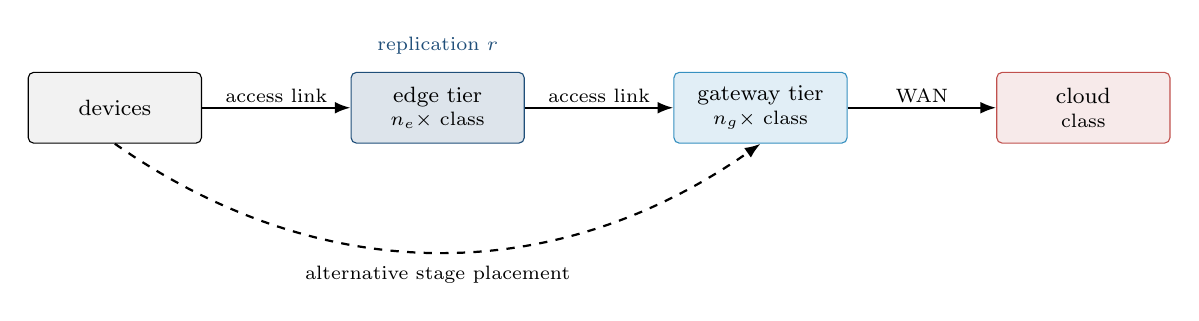
\begin{tikzpicture}[
  font=\footnotesize,
  box/.style={draw, rounded corners=2pt, minimum height=9mm, minimum width=22mm,
              align=center, inner sep=2pt},
  arr/.style={-{Latex[length=2mm]}, thick},
  lbl/.style={font=\scriptsize, midway, above=0.5mm, inner sep=0pt}]
\node[box, fill=black!5] (dev) at (0,0) {devices};
\node[box, fill=edgec!15, draw=edgec] (edge) at (4.1,0)
     {edge tier\\[-1pt]\scriptsize $n_e\times$ class};
\node[box, fill=gwc!15, draw=gwc] (gw) at (8.2,0)
     {gateway tier\\[-1pt]\scriptsize $n_g\times$ class};
\node[box, fill=cloudc!12, draw=cloudc] (cl) at (12.3,0)
     {cloud\\[-1pt]\scriptsize class};
\draw[arr] (dev) -- node[lbl] {access link} (edge);
\draw[arr] (edge) -- node[lbl] {access link} (gw);
\draw[arr] (gw) -- node[lbl] {WAN} (cl);
\draw[arr, dashed] (dev.south) to[out=-35, in=-145]
      node[font=\scriptsize, midway, below=0.5mm] {alternative stage placement} (gw.south);
\node[font=\scriptsize, text=edgec, above=1mm of edge] {replication $r$};
\end{tikzpicture}

\vspace{6mm}
\noindent\makebox[\linewidth][l]{\textbf{b}}\\[1mm]
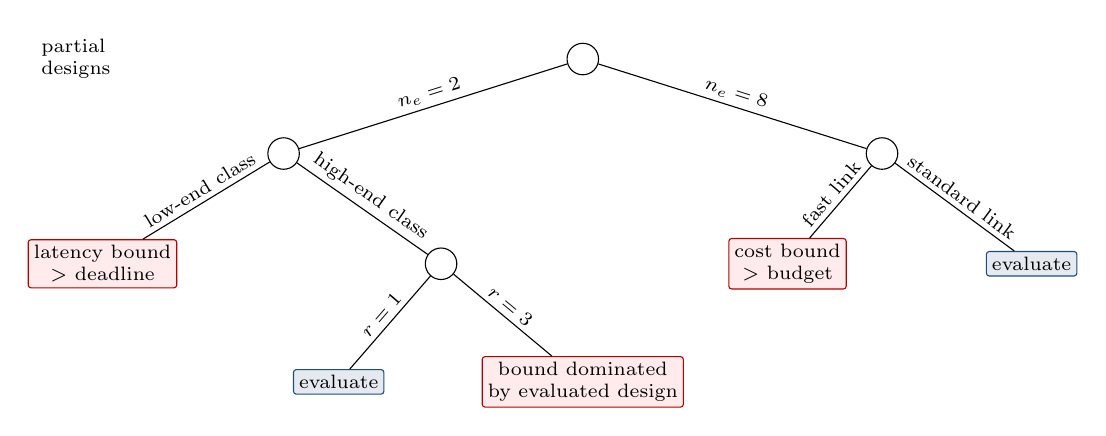
\begin{tikzpicture}[
  font=\scriptsize,
  n/.style={circle, draw, minimum size=4mm, inner sep=0pt},
  pr/.style={rectangle, draw=red!70!black, fill=red!8, rounded corners=1pt,
             align=center, inner sep=2pt},
  ev/.style={rectangle, draw=edgec, fill=edgec!12, rounded corners=1pt,
             align=center, inner sep=2pt},
  e/.style={-, thin}, el/.style={font=\scriptsize, midway, sloped, above=-0.5mm}]
\node[n] (root) at (7,3.6) {};
\node[n] (a) at (3.2,2.4) {}; \node[n] (b) at (10.8,2.4) {};
\draw[e] (root) -- node[el] {$n_e=2$} (a);
\draw[e] (root) -- node[el] {$n_e=8$} (b);
\node[pr] (p1) at (0.9,1.0) {latency bound\\$>$ deadline};
\node[n]  (c)  at (5.2,1.0) {};
\draw[e] (a) -- node[el] {low-end class} (p1);
\draw[e] (a) -- node[el] {high-end class} (c);
\node[ev] (e1) at (3.9,-0.5) {evaluate};
\node[pr] (p2) at (7.0,-0.5) {bound dominated\\by evaluated design};
\draw[e] (c) -- node[el] {$r=1$} (e1);
\draw[e] (c) -- node[el] {$r=3$} (p2);
\node[pr] (p3) at (9.6,1.0) {cost bound\\$>$ budget};
\node[ev] (e2) at (12.7,1.0) {evaluate};
\draw[e] (b) -- node[el] {fast link} (p3);
\draw[e] (b) -- node[el] {standard link} (e2);
\node[font=\scriptsize, anchor=west] at (0.0,3.6)
     {\begin{tabular}{@{}l@{}}partial\\designs\end{tabular}};
\end{tikzpicture}
\caption{\textbf{Exploration by elimination.} \textbf{a}, Architecture template: the
number and class of edge nodes and gateways, the class of the cloud instance, the access
link class, the replication factor of the ingest stage and the placement of the
processing stages are all design decisions. \textbf{b}, Each node of the traversal is a
partially specified architecture. It is discarded when an optimistic bound on a
constrained quantity already violates its limit (red), or when its optimistic objective
vector is dominated by an architecture that has already been evaluated (red); only
designs that survive to a leaf reach the expensive evaluator (blue).}
\label{fig:ce:concept}
\end{figure*}

%% ---------------------------------------------------------------- Table 1
\begin{table*}[!htbp]
\centering
\caption{\textbf{Positioning with respect to the closest prior work.} ``Partial-design
pruning'' denotes discarding incomplete designs before completing and evaluating them;
``contention-aware'' denotes objectives that depend on resource utilisation rather than
accumulating over decisions.}
\label{tab:ce:prior}
\scriptsize
\setlength{\tabcolsep}{3.5pt}
\begin{tabular}{@{}p{3.2cm}cp{2.2cm}ccccc@{}}
\toprule
Work & Year & System class & Obj. & Exact front & Partial-design & Contention- &
Real \\
 & & & & & pruning & aware & measurements \\
\midrule
Blickle et al.\cite{blickle1998system} & 1998 & embedded synthesis & 2 & no & no & no & no \\
Lukasiewycz et al.\cite{lukasiewycz2008symbolic} & 2008 & embedded synthesis & $n$ & no &
  SAT-based & no & no \\
Neubauer et al.\cite{neubauer2018exact} & 2018 & heterogeneous MPSoC & 3 & yes & symbolic &
  no & no \\
Kouloumpris et al.\cite{kouloumpris2024optimization} & 2024 & edge/hub/cloud & 1 &
  yes (BILP) & solver & no & UAV case \\
Sedghani et al.\cite{sedghani2024space4aid} & 2024 & computing continuum & 1 & no & no &
  partly & yes \\
CompDSE\cite{saadatmand2025compdse} & 2025 & industrial dCPS & perf. & --- & none & yes &
  traces \\
Kouloumpris et al.\cite{kouloumpris2026reliability} & 2026 & edge/hub/cloud & 2 &
  yes (BILP) & solver & no & case study \\
\textbf{This work} & 2026 & heterogeneous edge--cloud CPS & \textbf{4} & \textbf{yes} &
  \textbf{bounds} & \textbf{yes} & \textbf{yes} \\
\bottomrule
\end{tabular}
\end{table*}

\input{sections_ce/02_results_ce}

%% ---------------------------------------------------------------- Figures 2-7
\begin{figure}[!htbp]
\centering

\includegraphics[width=\linewidth]{figures/funnel.pdf}
\caption{\textbf{Architectures are removed before they are evaluated.} Raw design space,
survivors after structural and after bound-based elimination, and the number of
architectures actually handed to the evaluator, for four design-space scales and three
workload classes (logarithmic scale).}
\label{fig:ce:funnel}
\end{figure}

\begin{figure}[!htbp]
\centering
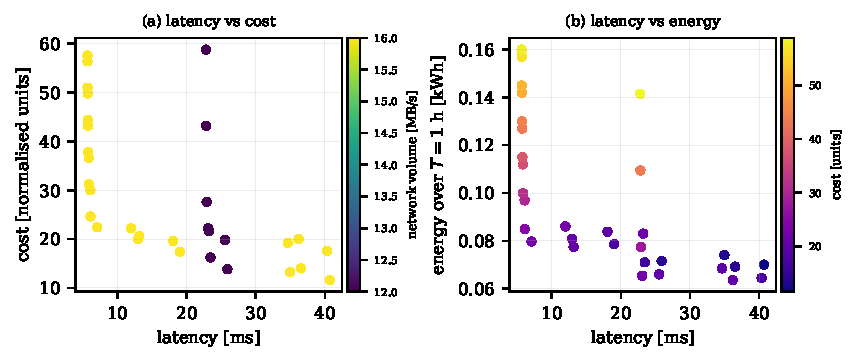
\includegraphics[width=\linewidth]{figures/pareto.pdf}
\caption{\textbf{The recovered set of optimal trade-offs.} Exact Pareto front on the
$51\,840$-candidate space for the telemetry workload. \textbf{a}, latency versus cost,
colour encodes network volume. \textbf{b}, latency versus energy over a one-hour horizon,
colour encodes cost.}
\label{fig:ce:pareto}
\end{figure}

\begin{figure}[!htbp]
\centering

\includegraphics[width=0.7\linewidth]{figures/crossover.pdf}
\caption{\textbf{The saving converts into time when evaluation is expensive.} Speed-up
over exhaustive enumeration projected from measured evaluation counts and measured
overheads as a function of the cost of one design-point evaluation. The dotted line marks
the measured cost of the discrete-event evaluator.}
\label{fig:ce:crossover}
\end{figure}

\begin{figure}[!htbp]
\centering

\includegraphics[width=\linewidth]{figures/hv_budget.pdf}
\caption{\textbf{Budget-matched stochastic exploration.} Hypervolume ratio against the
exhaustive front on the $51\,840$-candidate space over 20 seeds. Grey, random search;
blue, NSGA-II. The red line marks the exact front recovered by the proposed method.}
\label{fig:ce:hv}
\end{figure}

\begin{table}[!htbp]
\centering
\caption{\textbf{Budget-matched comparison.} Medians over 20 seeds at a budget of 1000
full evaluations; the full budget sweep is in Supplementary Tables~S1--S3.}
\label{tab:ce:base}
\scriptsize
\begin{tabular}{lllrrrrr}
\toprule
scale & workload & method & evals & recall & HV ratio & IGD$^{+}$ & time [s] \\
\midrule

\multirow{4}{*}{S2} & \multirow{4}{*}{telemetry} & exhaustive & 3\,888 & 1.000 & 1.000 & 0.0000 & 0.044 \\
 & & random ($B$=1000) & 1000 & 0.259 & 0.927 & 0.0388 & 0.014 \\
 & & NSGA-II ($B$=1000) & 1000 & 0.926 & 0.999 & 0.0002 & 0.147 \\
 & & \textbf{HCA-DSE} & \textbf{44} & \textbf{1.000} & \textbf{1.000} & \textbf{0.0000} & 0.036 \\
\midrule
\multirow{4}{*}{S2} & \multirow{4}{*}{control} & exhaustive & 3\,888 & 1.000 & 1.000 & 0.0000 & 0.042 \\
 & & random ($B$=1000) & 1000 & 0.240 & 0.922 & 0.0377 & 0.014 \\
 & & NSGA-II ($B$=1000) & 1000 & 0.800 & 0.999 & 0.0030 & 0.160 \\
 & & \textbf{HCA-DSE} & \textbf{37} & \textbf{1.000} & \textbf{1.000} & \textbf{0.0000} & 0.035 \\
\midrule
\multirow{4}{*}{S2} & \multirow{4}{*}{sensing} & exhaustive & 3\,888 & 1.000 & 1.000 & 0.0000 & 0.029 \\
 & & random ($B$=1000) & 1000 & 0.250 & 0.897 & 0.0626 & 0.010 \\
 & & NSGA-II ($B$=1000) & 1000 & 0.875 & 1.000 & 0.0017 & 0.182 \\
 & & \textbf{HCA-DSE} & \textbf{26} & \textbf{1.000} & \textbf{1.000} & \textbf{0.0000} & 0.016 \\
\midrule
\multirow{4}{*}{S3} & \multirow{4}{*}{telemetry} & exhaustive & 34\,560 & 1.000 & 1.000 & 0.0000 & 0.308 \\
 & & random ($B$=1000) & 1000 & 0.032 & 0.732 & 0.1147 & 0.011 \\
 & & NSGA-II ($B$=1000) & 1000 & 0.500 & 0.946 & 0.0454 & 0.145 \\
 & & \textbf{HCA-DSE} & \textbf{50} & \textbf{1.000} & \textbf{1.000} & \textbf{0.0000} & 0.138 \\
\midrule
\multirow{4}{*}{S3} & \multirow{4}{*}{control} & exhaustive & 34\,560 & 1.000 & 1.000 & 0.0000 & 0.265 \\
 & & random ($B$=1000) & 1000 & 0.000 & 0.725 & 0.1189 & 0.010 \\
 & & NSGA-II ($B$=1000) & 1000 & 0.648 & 0.984 & 0.0236 & 0.147 \\
 & & \textbf{HCA-DSE} & \textbf{41} & \textbf{1.000} & \textbf{1.000} & \textbf{0.0000} & 0.125 \\
\midrule
\multirow{4}{*}{S3} & \multirow{4}{*}{sensing} & exhaustive & 34\,560 & 1.000 & 1.000 & 0.0000 & 0.266 \\
 & & random ($B$=1000) & 1000 & 0.000 & 0.658 & 0.1569 & 0.010 \\
 & & NSGA-II ($B$=1000) & 1000 & 0.741 & 0.951 & 0.1677 & 0.175 \\
 & & \textbf{HCA-DSE} & \textbf{43} & \textbf{1.000} & \textbf{1.000} & \textbf{0.0000} & 0.085 \\
\bottomrule
\end{tabular}

\end{table}

\begin{figure}[!htbp]
\centering

\includegraphics[width=0.7\linewidth]{figures/scalability.pdf}
\caption{\textbf{The design space is never materialised.} Expanded partial designs and
full evaluations against the raw design-space size, over five orders of magnitude.}
\label{fig:ce:scal}
\end{figure}

\begin{table}[!htbp]
\centering
\caption{\textbf{Independent deployment validation.} Analytical predictions against
measured run means over 36 architectures and 108 runs with the model frozen beforehand.
Pair agreement is the share of architecture pairs whose measured order matches the
predicted order among pairs separated by more than $25\%$. ALL pools workloads.}
\label{tab:ce:testbed}
\scriptsize
\small
\begin{tabular}{lrrrrr}
\toprule
workload & $n$ & MAPE [\%] & Spearman $\rho$ & agreement $>25\%$ & pairs \\
\midrule
telemetry & 12 & 17.8 & 0.776 & 0.895 & 38 \\
control & 12 & 12.0 & 0.865 & 0.886 & 44 \\
sensing & 12 & 46.3 & 0.921 & 0.913 & 23 \\
ALL & 36 & 25.4 & 0.967 & 0.978 & 498 \\
\bottomrule
\end{tabular}

\end{table}

\begin{figure}[!htbp]
\centering

\includegraphics[width=0.62\linewidth]{figures/testbed.pdf}
\caption{\textbf{Predicted against measured latency.} Analytical latency versus the
median of three measured mean latencies on the independent containerised deployment. Open
markers denote architectures whose repeated means differ by a factor of $1.5$ or more.}
\label{fig:ce:testbed}
\end{figure}

\input{sections_ce/03_discussion_ce}
\section*{Methods}
\label{sec:ce:methods}

\subsection*{Architecture template and design space}
The template has four tiers --- devices, edge nodes, gateways and cloud --- and three
application stages per request. Pre-processing runs on the edge or gateway tier,
aggregation always on the gateway tier, and analytics on the edge tier or in the cloud;
which variant is instantiated is a design decision. A compute class is a tuple
$(C,M,P^{\mathrm{idle}},P^{\mathrm{peak}},c)$ of capacity [MIPS], memory [MB], idle and
peak power [W] and normalised cost; a link class is $(B,\tau^{\mathrm{prop}},e,c)$ of
bandwidth [Mb/s], propagation delay, transfer energy [J/MB] and cost per attached node.
The gateway-to-cloud connection is fixed infrastructure ($200$\,Mb/s, $20$\,ms) and is
not a design variable. An architecture is
\begin{equation}
x=\big(n_e,\ \kappa_e,\ n_g,\ \kappa_g,\ \ell,\ \kappa_c,\ r,\ \pi\big),
\label{eq:ce:decision}
\end{equation}
with node counts $n_e,n_g$, classes $\kappa_e,\kappa_g,\kappa_c$, link class $\ell$,
replication factor $r$ of the ingest stage and placement policy $\pi$. The design space is
the Cartesian product $\X=D_1\times\dots\times D_k$, $k=8$. Four scales
(S1--S4) and three workload classes --- high-rate telemetry, deadline-dominated real-time
control and payload-dominated sensing --- are used throughout; their domains and
parameters are listed in Supplementary Tables~S8--S10.

\subsection*{Evaluation model}
With $t(i)$ the tier executing stage $i$, $N_t$ its node count and $C_t$ the per-node
capacity of its class, the offered load and utilisation are
$\Theta_t=\sum_{i:t(i)=t}\Lambda w_i\mu_i$ and $\rho_t=\Theta_t/(N_tC_t)$, where
$\Lambda$ is the system arrival rate and $\mu_i=r$ for the ingest stage and $1$
otherwise. A tier is modelled as one queueing station with the aggregate capacity of its
nodes, deterministic service and Poisson arrivals, so that
\begin{equation}
L(x)=\sum_{i=1}^{3}\frac{w_i}{C_{t(i)}}
+\sum_{i=1}^{3}\frac{w_i}{C_{t(i)}}\cdot\frac{\rho_{t(i)}}{2\,(1-\rho_{t(i)})}
+\sum_{(s,\ell)\in\mathcal{H}(x)}\Big(\frac{8s}{B_\ell}+\tau^{\mathrm{prop}}_\ell\Big),
\label{eq:ce:latency}
\end{equation}
where $\mathcal{H}(x)$ is the set of hops implied by the policy and the replication
factor. The middle term is the contention-dependent one. The aggregation is an
approximation --- a tier of $N_t$ single-server nodes is an M/D/$c$ system rather than an
M/D/1 system with $c$-fold capacity, and the approximation is optimistic --- kept
deliberately because it is the coarsest form that still makes latency depend on
utilisation and remains monotone in the design variables. Both the discrete-event
evaluator and the physical testbed implement per-node servers, so its cost is measured
rather than assumed. Energy over a horizon $T=1$\,h combines idle and load-proportional
compute power with transfer energy; cost sums node and link coefficients; network volume
is the per-second byte flow. Feasibility requires $\rho_t\le0.85$ on every used tier,
memory and bandwidth to fit, and the latency, cost and energy budgets to hold. Full
expressions are in Supplementary Note~2.

\subsection*{Admissible bounds}
Write $\C(p)$ for the completions of a partial design $p$. A bound $\LB_i$ is admissible
if $\LB_i(p)\le f_i(x)$ for all $x\in\C(p)$. Two constructions are used.

\emph{Term-wise relaxation.} If $f_i(x)=\sum_{t\in T_i}\varphi_t(x)$ with
$\varphi_t\ge0$ and $\underline{\varphi}_t(p)=\min_{x\in\C(p)}\varphi_t(x)$, then
$\LB_i(p)=\sum_t\underline{\varphi}_t(p)$ is admissible, because each term is bounded
below independently. The minima are taken per term, so the combination realising them
need not correspond to any completion; the bound is optimistic but valid. Every term of
the model is monotone in each free variable, so each minimum is attained at a domain
endpoint and is read from a table of precomputed extrema in constant time.

\emph{Exactness on determined terms.} If the variables a term depends on are already
assigned, the term is constant on $\C(p)$ and its exact value may replace the relaxed
one, which preserves admissibility and tightens the bound. The decision order places the
determinants of tier utilisation --- node counts, classes, replication and policy ---
before the remaining variables, so the waiting term of \eqref{eq:ce:latency} becomes
exact early in the traversal instead of being relaxed to zero. This is what makes a
contention-dependent objective usable without assignment monotonicity. If the
determinants are fixed and $\rho_t\ge1$, no completion has finite latency and the bound
is $\infty$, which is admissible.

\subsection*{Pruning rules and exactness}
Three rules are applied at each node of the prefix tree. \emph{Structural}: the
well-formedness predicate $\sigma$ (gateways do not outnumber edge nodes, replication
does not exceed the edge count, replication is undefined for policies that place ingest
off the edge tier) depends only on assigned variables and cannot be repaired by later
assignments, so a violation eliminates all completions. It defines the search space
rather than following from the constraints, and the exhaustive baseline applies the same
predicate. \emph{Feasibility}: if an admissible bound on a constrained quantity exceeds
its limit, no completion is feasible. \emph{Dominance}: if an evaluated feasible
architecture $y$ satisfies $F(y)\preceq \LB(p)$, then every completion of $p$ is
dominated by $y$ and none can be Pareto-optimal. Together with admissibility these give
front preservation: the non-dominated set returned equals the exact Pareto front of the
model in objective space. Proofs are in Supplementary Note~1. Two consequences are used
in the experiments: the guarantee is order-independent, so traversal order affects
efficiency only; and it is stated in objective space, so architectures sharing an
objective vector may be represented once.

\subsection*{Verification of correctness}
Theoretical correctness and implementation correctness are checked separately. Bound
admissibility is verified exhaustively on the smallest scale --- every partial design
against every completion, for all three workloads. For every partial design that the
implementation prunes, all of its completions are enumerated and checked against the
claim of the rule that discarded it. Equality with the exhaustive front is re-checked on
S1--S3 for every pruning variant as a regression test.

\subsection*{Baselines}
Exhaustive enumeration provides ground truth on S1--S3. Random search and
NSGA-II\cite{deb2002nsga2} (pymoo\cite{blank2020pymoo}, population $40$, SBX crossover,
polynomial mutation, integer repair) run at matched budgets of $100$, $250$, $500$ and
$1000$ full evaluations with $20$ seeds each; budgets are charged to actual evaluator
calls, including infeasible ones. An independent exact baseline encodes the finite
evaluated relation and solves for the non-dominated set with an SMT
solver\cite{demoura2008z3}; it requires the full table to be built first and therefore
consumes one evaluator call per structurally valid candidate. Recall and precision are
computed on sets of objective vectors, hypervolume\cite{zitzler1999hv} is normalised by
the exhaustive front, and IGD$^{+}$\cite{ishibuchi2015igdplus} uses that front as
reference, following the guidance on indicator choice in ref.~\citenum{audet2021indicators}.
Stochastic baselines are compared with the one-sided Mann--Whitney
$U$ test\cite{mann1947whitney} and Cliff's $\delta$\cite{cliff1993delta}, reported
unadjusted and treated as exploratory.

\subsection*{Discrete-event evaluator}
A higher-fidelity evaluator simulates each design with multi-server tiers, explicit link
contention, deterministic service and Poisson arrivals. It serves two purposes: as an
internal reference for the accuracy of the analytical model, and as the anchor of the
evaluation-cost analysis, at a measured $\DesCostMs$\,ms per design point averaged over
$40$ designs.

\subsection*{Containerised deployment}
Each edge node, gateway and cloud instance is a separate container limited to one CPU, so
that a node behaves as the single server the model assumes at node level. Services are
written in Go and share one binary: a request carries a plan of the remaining stages,
each node consumes CPU work equal to $w_i/C_t$ and forwards the remainder with the real
payload to the next hop. Links are shaped per node with \texttt{tc netem}
\cite{hemminger2005netem} using the delay and rate of the link class under test, with a
wide-area profile on the cloud hop; shaping is applied in the forward direction of each
hop, matching the one-way transfers counted by the model. Replication is emulated
faithfully: $r$ replicas execute the ingest stage in parallel and carry the
synchronisation payload, and the remainder of the chain executes once. A load generator
produces Poisson arrivals, $900$ requests per run of which $150$ are discarded as warm-up.
Thirty-six architectures --- Pareto-optimal, dominated and near-boundary --- were selected
subject to fitting on one machine ($\le4$ edge nodes, $\le2$ gateways), and each was run
three times. The analytical model was frozen before this round.

\subsection*{Reproducibility}
The implementation is Python 3 with NumPy, SciPy and pymoo; the deployment services are
Go under Docker Compose. Every figure and every numeric table in this paper, main and
supplementary, is generated from the raw result files by a single script, so no number is
transcribed by hand.

\section*{Data availability}
All result files underlying the figures and tables --- exploration funnels, budget sweeps
with per-seed metrics, ablations, scalability sweeps, discrete-event comparisons and the
$108$ measured deployment runs --- are included in the replication package accompanying
this submission.

\section*{Code availability}
The exploration method, the analytical and discrete-event evaluators, the baselines, the
containerised deployment and the verification tests are included in the same package,
together with the single script that regenerates every display item from the raw results.

\section*{Author contributions}
N.T. designed the method, implemented the software and the deployment, ran the
experiments and wrote the manuscript. V.T. contributed to the system model and the
experimental design and reviewed the manuscript.

\section*{Competing interests}
The authors declare no competing interests.


\bibliographystyle{elsarticle-num}
\bibliography{refs}

\end{document}
